\documentclass[10pt,a4paper]{article}
\usepackage[utf8]{inputenc}
\usepackage[italian]{babel}
\usepackage{amsmath}
\usepackage{amsfonts}
\usepackage{amssymb}
\usepackage{graphicx}
\usepackage{gensymb}
\usepackage[left=2cm,right=2cm,top=2cm,bottom=2cm]{geometry}
\newcommand{\rem}[1]{[\emph{#1}]}

\author{Gruppo BN \\ Federico Belliardo, Lisa Bedini, Marco Costa}
\title{Esperienza 12: Flip-Flop e contatori}

\begin{document}
\maketitle

\section{Flip-Flop D-Latch}
Si è realizzato un circuito flip-flop di tipo D-Latch, come mostrato in figura \ref{D-Latch} utilizzando le porte NAND di due integrati. L'ingresso D che corrisponde al dato da memorizzare è stato collegato all'impulsatore realizzato con Arduino Nano (in particolare a Y1 o a Y2?), e l'Enable è collegato alla tensione positiva attraverso uno switch manuale (inserire resistenza di pull-up?). La tensione di lavoro durante tutta l'esperienza è stata fissata a: $V_{CC} = $.\\

%Riportiamo in tabella \ref{stati} le configurazioni del R-S NAND Latch per maggior chiarezza %delle spiegazioni successive:

\begin{figure}
\centering
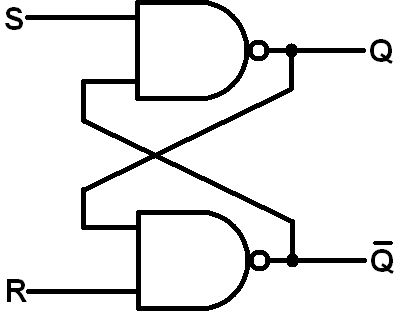
\includegraphics[scale=0.5]{latchNand.png}
\caption{R-S NAND Latch.\label{fig:latch}}
\end{figure}

\begin{figure}
\centering
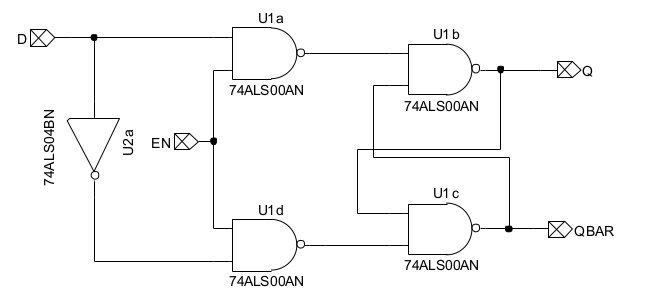
\includegraphics[scale=0.7]{flipflopDlatch.png}
\caption{Circuito  D-Latch NAND.\label{fig:circuito}}
\end{figure}

In figura \ref{segue} si vede come il segnale $Q(t)$ in uscita dal flip-flop segua l'ingresso quando enable è alto riproducendo la tabella \ref{stati2}.\\

\begin{table}[!htb]
\centering
\begin{tabular}{|c|c|c|c|c|}
\hline 
EN & D & S & R & Q\\ 
\hline 
1 & 1 & 0 & 1 & 1\\ 
\hline 
1 & 0 & 1 & 0 & 0\\ 
\hline 
0 & 1 & 1 & 1 & Hold\\ 
\hline 
0 & 0 & 1 & 1 & Hold\\ 
\hline 
\end{tabular}
\caption{Tabella degli stati per un Flip-Flop NAND. \label{stati2}}
\end{table}


Commutando manualmente lo switch e impostando dunque $EN = 0$ il flip flop rimane congelato nello stato in cui si trovava prima della commutazione.
Perché il valore che il flip-flop memorizza sia deterministico è necessario che la commutazione dello switch non avvenga durante gli hold-time e setup-time del latch. In figure \ref{cong1} e \ref{cong2} si vede il flip-flop congelato nei due stati. Quando il bit di enable è disattivato entrambe le uscite dei NAND del primo livello sono a 1 pertanto il latch è nello stato di hold.\\

Essendo il latch costruito con delle porte NAND ho una situazione di instabilità quando gli ingressi delle porte sul secondo livello sono entrambe a 0. Questo può succedere solo se gli ingressi di tutte le porte sul primo livello sono 1. IL NOT evita questa situazione.\\
L'enable è attivo alto. Cioè quando $enable = 0$ ho permanenza dello stato, infatti gli ingressi al secondo livello dei NAND sono sicuramente a 1. mentre posso avere evoluzione dello stato se il bit $enable = 1$.\\

Si sono misurati i tempi di ritardo sulla salita e discesa del flip-flop (quando è abilitato) essi sono risultati asimmetrici. Le misure sono riportate nella tabella \ref{ritardo}.

\begin{table}[!htb]
\centering
\begin{tabular}{|c|c|}
\hline 
$t_{LH}$ (ns) & $t_{HL}$ (ns)\\
\hline
tempo 1 & tempo 2\\
\hline
\end{tabular}
\caption{Misure dei tempi di ritardo in salita e discesa per il Flip-Flop. \label{stati2}}
\end{table}

%TODO -> dire se sono in attesa con quanto atteso e spiegare perchè sono asimmetrici.

\section{Divisori di frequenza}
Si è realizzato un contatore a 4 bit come in figura \ref{contatore} connettendo l'uscita Q del primo JK (FF1) al clock del secondo JK (FF2),i restanti JK sono già interconnessi all'interno del package. Si vogliono utilizzare tutti i JK in modalità Toggle, cioè in modo che oscillino tra lo stato 0 e 1 alla transizione basso-alto del clock (per costruzione). Per fare cioò è necessario che l'ingresso J di ognuno dei flip-flop sia impostato a 1, questa configurazione è realizzata ponendo $R_0$ a terra e $R_1$ flottante (per il momento).\\
%perchè cose flottanti sono uguali a 1 di default??
Infatti la configurazione toggle del JK si ottiene se $J = 1$ e $K = 1$ dunque con K flottante questo è sempre uguale a 1, se uno egli ingressi del NAND è forzato a 0 la sua uscita sarà sempre 1 e sono quindi nella richiesta per i JK.\\  
Poiché la transizione del valore di uscita Q di ognuno degli FF avviene con una frequenza dimezzata rispetto a quella del clock, le varie uscite $Q_i(t)$ oscillano con frequenze $\frac{1}{2}, \frac{1}{4, \frac{1}{8}, \frac{1}{16}$ in quanto l'uscita $Q_i$ di un FF è il clock del successivo.\\
Ogni uscita $Q_i$ è stata collegata a terra attraverso un LED e una resistenza (per limitare la corrente sul led). Questo e l'accorgimento di impostare un clock per il FF1 di 1 Hz (generato con Arduino) rende osservabili ad occhio nudo le transizioni.\\
Interpretando il bit più a sinistra come bit meno significativo (1 per LED acceso e 0 per LED spento) si ottiene la rappresentazione fisica dei numeri da 0 a 15 in binario.\\

\begin{figure}
\centering
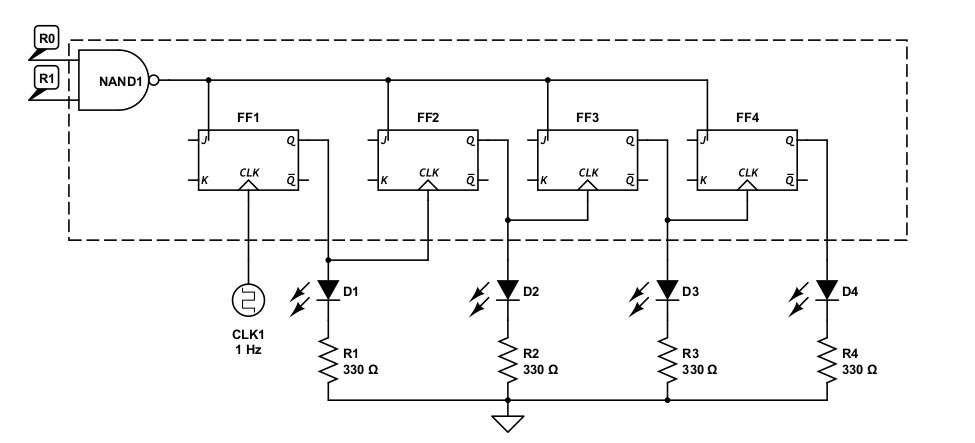
\includegraphics[scale=0.5]{divisore.png}
\caption{Contatore a 4 bit.\label{fig:contatore}}
\end{figure}

Si è inviato in ingresso (sempre con Arduino) un segnale di frequenza $f = kHz$, si sono misurate le frequenze dei segnali $Q_i$ e i tempi di ritardo per la salita e la discesa rispetto al clock, definiti come differenza temporale i punti in cui i due segnali raggiungono la metà del rispettivo valore massimo.\\

\begin{table}[!htb]
\centering
\begin{tabular}{|c|c|c|c|c|}
\hline 
• & $T (ms)$ & $f (kHz)$ & $t_{HL}$ & $t_{LH}$ \\ 
\hline 
$Q_2$ & • & • & • & • \\ 
\hline 
$Q_2$ & • & • & • & • \\ 
\hline 
$Q_3$ & • & • & • & • \\ 
\hline 
$Q_4$ & • & • & • & • \\ 
\hline 
\end{tabular} 
\caption{Misure di frequenza e tempi di propagazione per il divisore. \label{misureDivisore}}
\end{table}

I tempi di ritardo misurati sono tempi di propagazione attraverso la rete dei flip-flop e dalle misure eseguite aumentano linearmente con il numero di porte del circuito. Il tempo di propagazione da \emph{low} a \emph{high} è sistematicamente più alto di circa $\Delta t = ... ns$, come si può vedere nella tabella \ref{misureDivisore}.\\ 
%I tempi di propagazione sono compatibili con il numero di porte che ci sia aspetta essere in ogni latch?
%TODO - Eseguire un fit per la linearità

Si vuole realizzare un contatore decadico sincrono, cioè attivare il reset quando il contatore raggiunge il valore 10. Per identificare il valore 10 sulle uscite $Q_i$ si esegue un NAND tra le uscite $Q_2$ e $Q_4$, che da un segnale basso non appena i due bit sono attivati per la prima volta (cioè si raggiunge il 10). \\
Il reset dei JK si ottiene per $J = 0$ e $K = 1$, dunque K viene sempre lasciato flottante
A questo punto sarebbe possibile fornire questo valore agli ingressi di reset del circuito, tuttavia per costruire un reset sincrono con il clock si utilizza un D-Latch.\\
Il bit di reset $R_1$ viene collagato ora a 1 attraverso una resistenza, il bit $R_2$ è collegato all'uscita negata del latch in modalità enabled. In questo modo l'uscita $\bar{Q}$ diventa 1 non appena si raggiunge 10 e sincronamente con il clock. Infine $\bar{Q}$ viene collegata al bit $R_2$ di reset e così si è realizzato il contatore decimale.\\
Se non è ancora stato raggiunto il 10 $Q = 1$, $\bar{Q} = 0$ e dunque tutti i FF sono in modalità toggle (J = 0 NAND 1 = 1, K =1 ) e il conteggio continua. Non appena $\bar{Q} = 1$ , cioè ho raggiunto il 10 l'uscita degli FF viene impostata a 0, infatti J = 1 NAND 1 = 0, K = 1 che sappiamo corrispondere al settaggio di $Q = 0$.

 

%TODO - Vedere se invertir il clock.
%Discutere il clock e discutere le caratteristiche - riportare le misure. 

\section{Shift register con D-Latch}

\section{Generatore di numeri casuali}

\end{document}







